\section{Sezione Utente}
\label{sec:sezUtente}

\subsection{Impostazioni di sistema}
Nella sezione superiore destra dell'interfaccia, cliccando sull'icona impostazioni 
\includegraphics[height=1.2em]{assets/settings_icon.png} apparirà il menu laterale delle impostazioni di sistema.
% \begin{figure}[H]
%   \centering
%   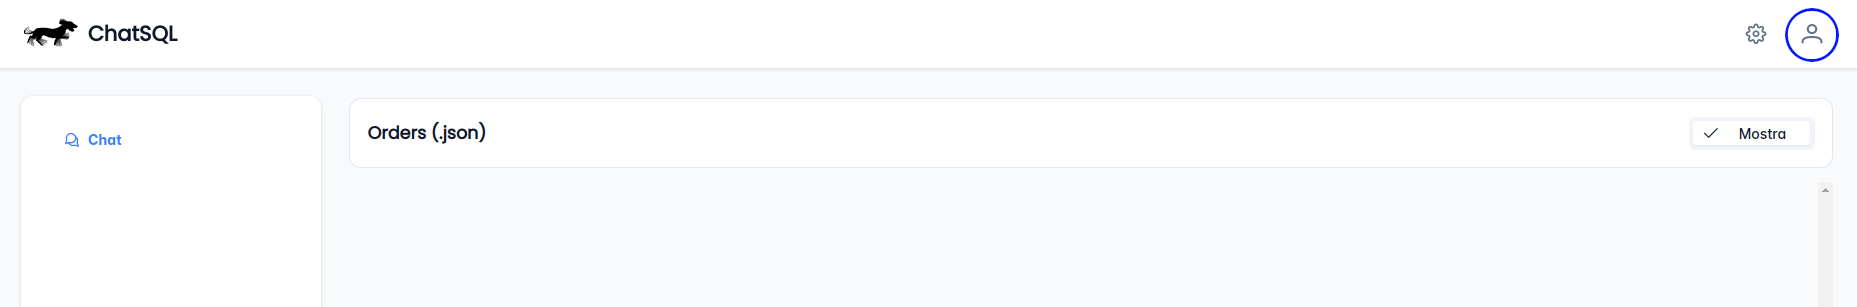
\includegraphics[width=1\textwidth]{assets/login_topbar.png}
%   \caption{Topbar con menu di autenticazione}
% \end{figure}
\begin{figure}[H]
  \centering
  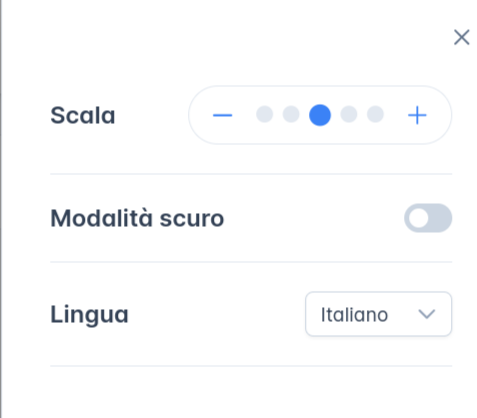
\includegraphics[width=0.50\textwidth]{assets/menu_config.png}
  \caption{Menu laterale delle impostazioni di sistema}
\end{figure}
\par Le impostazioni di sistema permettono di configurare le seguenti opzioni:
\begin{itemize}
  \item Scala: dimensioni del testo e della schermata;
  \item Modalità scuro: abilita o disabilita la modalità scura dell'interfaccia;
  \item Lingua: selezione della lingua dell'interfaccia tra Inglese e Italiano.
\end{itemize}
\par Le modifiche apportate verranno memorizzate automaticamente, e applicate alla successiava apertura dell'applicazione.